\section{Infrastruttura IT}
\subsection{Descrizione}
\subsection{Apparati Utilizzati}
\subsubsection{Descrizione}
\subsubsection{Data server}
Il database sarà collocato nel data server che conterrà anche le immagini di profilo degli utenti e quelle legate ai prodotti. 
\subsubsection{Application server}
\subsubsection{API server}
\subsubsection{Web server}
\subsection{Progetto di rete} 
Ho progettato la rete per la sede centrale dell'azienda usando il programma di simulazione Cisco Packet Tracer 8.0, nelle etichette da me inserite sono riportati gli indirizzi IP degni di nota e le informazioni relative alle 4 sottoreti create. Il file è stato caricato assieme a tutto il progetto nell'apposita repository creata su GitHub e \href{https://github.com/MauroPello/elaborato}{raggiungibile qui} \cite{GitHub}. 
\begin{sidewaysfigure}
    \centering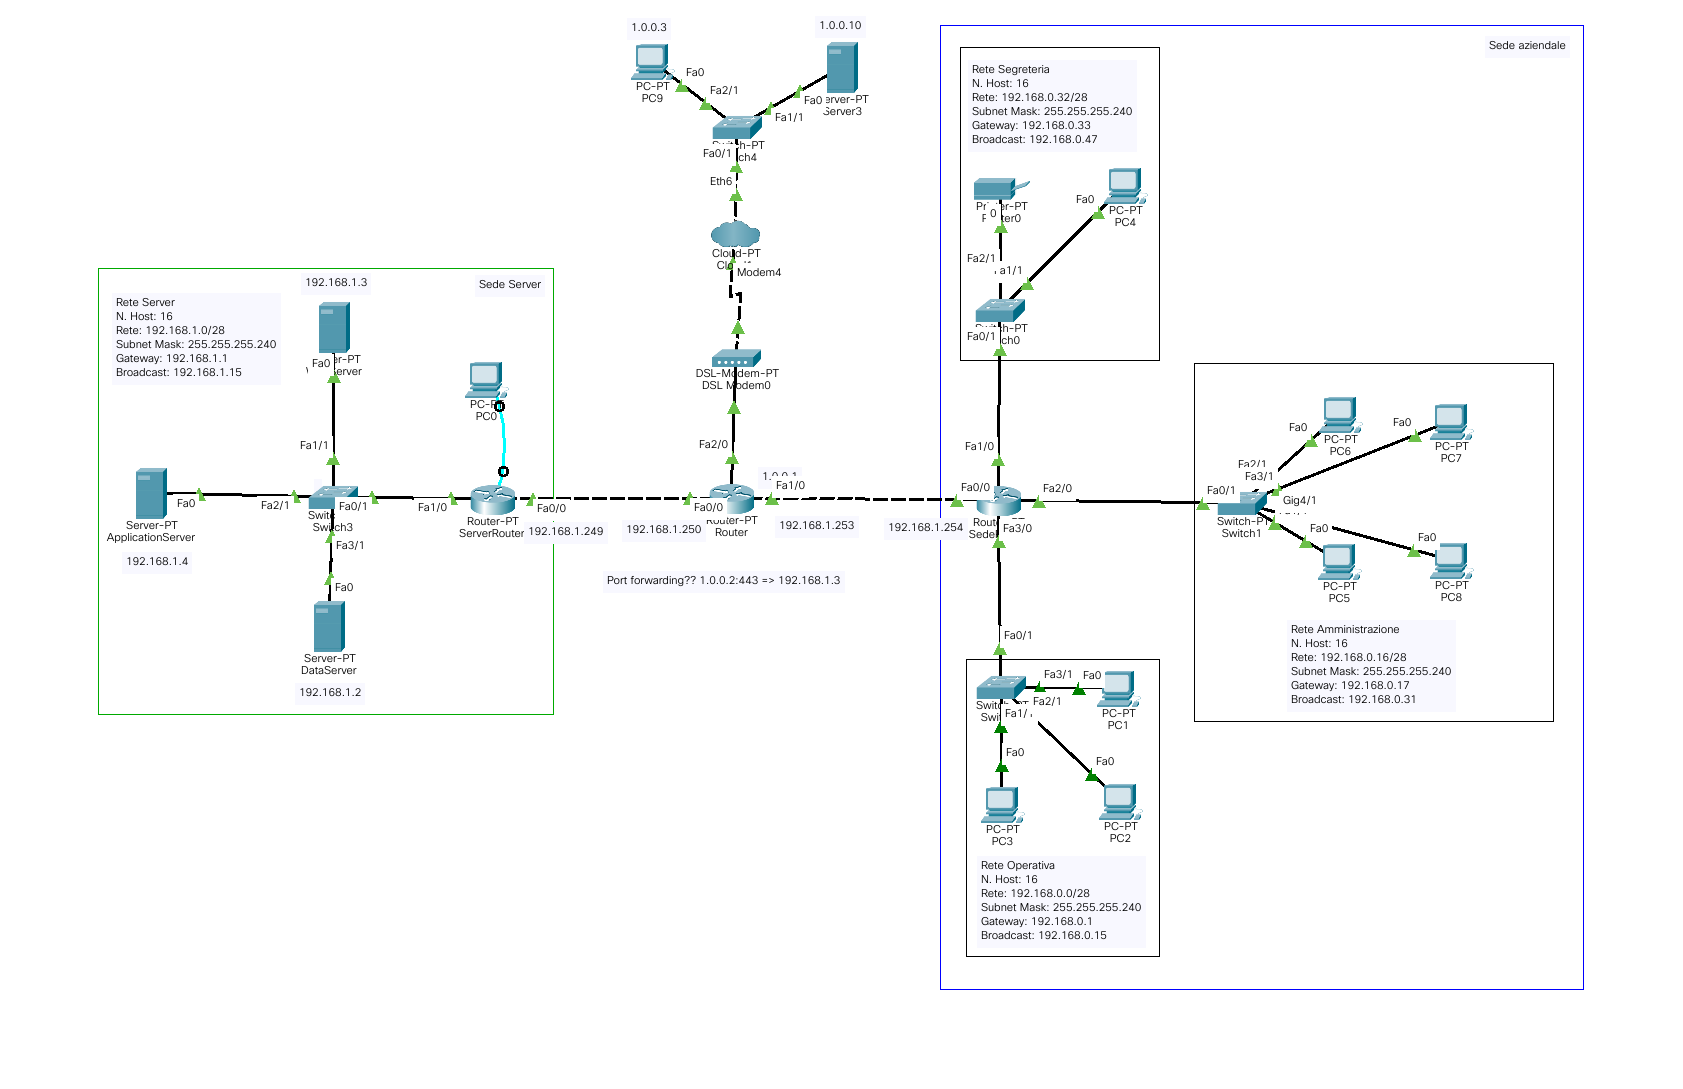
\includegraphics[scale=.48]{images/rete.png}
    \caption{Progetto della rete sviluppato con Cisco Packet Tracer 8.0}
\end{sidewaysfigure}
\clearpage